\documentclass[a4paper]{article}
\usepackage[utf8]{inputenc}
\usepackage{amsmath}
\usepackage{siunitx}
\usepackage[ngerman]{babel}
\usepackage{pgfplots}
\usepackage{hyperref}
\usepackage{pgfplotstable}
\usepackage[section]{placeins}
\usepackage{enumitem}
\usepackage{listings}
\usepackage{float}

%für Code
\usepackage{color} %red, green, blue, yellow, cyan, magenta, black, white
\definecolor{mygreen}{RGB}{28,172,0} % color values Red, Green, Blue
\definecolor{mylilas}{RGB}{170,55,241}
\lstset{language=Matlab,%
    %basicstyle=\color{red},
    breaklines=true,%
    morekeywords={matlab2tikz},
    keywordstyle=\color{blue},%
    morekeywords=[2]{1}, keywordstyle=[2]{\color{black}},
    identifierstyle=\color{black},%
    stringstyle=\color{mylilas},
    commentstyle=\color{mygreen},%
    showstringspaces=false,%without this there will be a symbol in the places where there is a space
    numbers=left,%
    numberstyle={\tiny \color{black}},% size of the numbers
    numbersep=9pt, % this defines how far the numbers are from the text
    emph=[1]{for,end,break},emphstyle=[1]\color{red}, %some words to emphasise
    %emph=[2]{word1,word2}, emphstyle=[2]{style},    
}


\pgfplotsset{compat=1.15}

\title{GPET\\ Auswertung Versuch 3\\ Gruppe 1}

\author{Jonas Otto\\ \href{mailto:jonas@jonasotto.com}{jonas@jonasotto.com} 
   \and Luca Krüger \\ \href{mailto:luca.krueger@uni-ulm.de}{luca.krueger@uni-ulm.de} }
\date{am 7. Mai 2018}

\begin{document}

\maketitle
\newpage

% \section{Vorbereitung}

% \subsection{Signaleigenschaften und Signalklassifikation}
% \subsubsection{Signalklassifikation}
% \begin{enumerate}[label=\alph*)]
% \item Harmonisch
% \item Deterministisch
% \item Stochastisch
% \item Periodisch
% \end{enumerate}

% \subsubsection{Harmonische Signale}
% $f=1\si{Hz}$, $T=1\si{s}$, $\phi_0=-\frac{\pi}{2}$
% % Diagramm: Vertikaler Strich bei 1Hz

% \subsubsection{Elektrische Signale}
% $\hat{x}=1\si{V}$, $x_{\textit{eff}}=\frac{1}{\sqrt{2}}\si{V}\approx 0.71\si{V}$, $x_{ss}=2\si{V}$, $\bar{x}\approx 0.3\si{V}$

% \subsection{Transformation in den Frequenzbereich}
% \subsubsection{Bandbreite}
% \begin{enumerate}[label=\alph*)]
% \item $f_1\approx 1000\si{Hz}$, $f_2\approx 2100\si{Hz}$, $B\approx 1100\si{Hz}$
% \item $f_1\approx 1000\si{Hz}$, $f_2\approx 1600\si{Hz}$, $B\approx 600\si{Hz}$
% \end{enumerate}

% \subsubsection{Darstellung im Frequenzbereich}
% % Diagramm: Vertikaler Strich bei 3Hz, 9Hz
% $A(t)=1\si{V} \cdot \cos{(2\pi \cdot 3\si{Hz} \cdot t)} + 0.5\si{V} \cdot \cos{(2\pi \cdot 9\si{Hz} \cdot t)}$

% \subsubsection{Matlab}
% \paragraph{i)}
% Command Window: Eingeben von Befehlen und Anzeige von Ausgaben.\\
% File Browser: \\
% Workspace: Zeigt aktuell definierte Variablen und dessen Typ und Wert an.\\
% Command History: Zeigt eine Liste aller ausgeführten Befehle an.
% \paragraph{ii)}
% Eingeben von \glqq temp\grqq in der Befehlszeile.
% \paragraph{iii)}
% \glqq doc fft\grqq
% \paragraph{iv)}
% m(1,[1:end])
% \paragraph{v)}
% [s, d] = fsummdiff(1,2)

% \subsubsection{FFT Auflösung}
% 8 Perioden, $t_{\textit{Messung}}=8\cdot \frac{1}{1500\si{Hz}}\approx 5.3\si{ms}$, Frequenzauflösung $f=\frac{1}{t_{\textit{Messung}}} = 187.5\si{Hz}$

% \subsection{Mehrfrequenzwahlverfahren}
% \subsubsection{MFV-Signale im Zeitbereich}
% $A(t)=\cos{(2\pi \cdot 697\si{Hz} \cdot t) + \cos{(2\pi \cdot 1209\si{Hz} \cdot t)}}$

% \subsubsection{MFV-Signale im Frequenzbereich}
% \begin{equation*}
%     X_k(k\cdot f_0) = \int^{T/2}_{-T/2} ( \cos{(2\pi \cdot 697\si{Hz} \cdot t) + \cos{(2\pi \cdot 1209\si{Hz} \cdot t)}} ) \cdot e^{-j \pi k f_0 t} \,\text{d}t
% \end{equation*}

% \subsubsection{Sprachsignale}
% Sprache: ca. $300\si{Hz}$ - $5\si{kHz}$\\
% Audio: ca. $20\si{Hz}$ - $20\si{kHz}$\\
% Die Töne beim Mehrfrequenzwahlverfahren liegen also im hörbaren Bereich.

\section{Versuchsauswertung}
\subsection{Messung harmonischer Signale}\label{sec:harmonische-signale}
\subsubsection{Einstellungen des Oszilloskopss}
Für den Einstieg wurde der interne Funktionsgenerator des Oszilloskops auf eine Frequenz von $697\si{\Hz}$ und einer Amplitude von $1\si{V}$ eingestellt und über Kanal$1$ des Oszilloskops überprüft.
Die Messung ergab eine Peak-to-Peak Spannung $V_{\text{pp}}=2\si{V}$, einen Effektivwert $V_{\textit{eff}}=\frac{1}{\sqrt{2}}V_{Amplitude}=0.7\si{V}$, ein Offset $V_{\textit{off}}=0\si{V}$ und eine Frequenz $f=\frac{1}{T}=697\si{Hz}$. In Abbildung \ref{fig:cursor-freq-ampl} ist abzulesen, dass der Mittelwert $V_m = \frac{V_{max}+V_{min}}{2}=V_{\textit{off}}=0\si{V}$ beträgt.

\begin{figure}[H]
    \centering
    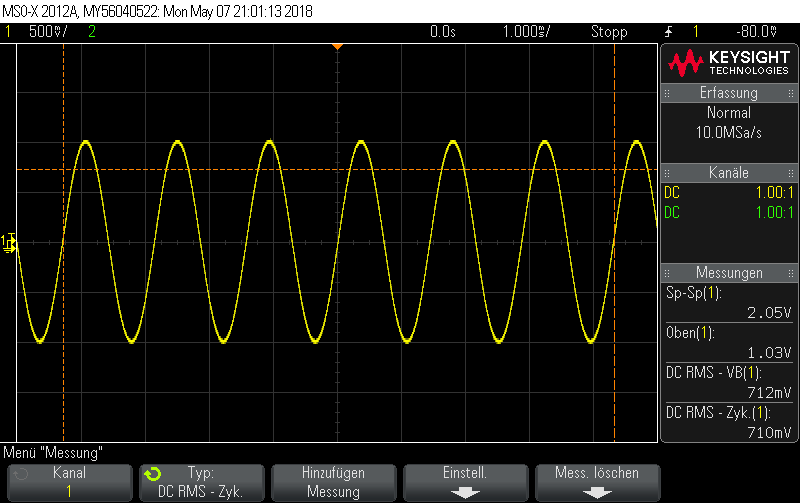
\includegraphics[width=0.8\textwidth]{aufgabe1_rms_meas.png}
    \caption{Bestimmung des Effektivwerts mit der Measure Funktion}
    \label{fig:rms-meas}
\end{figure}

\begin{figure}[H]
    \centering
    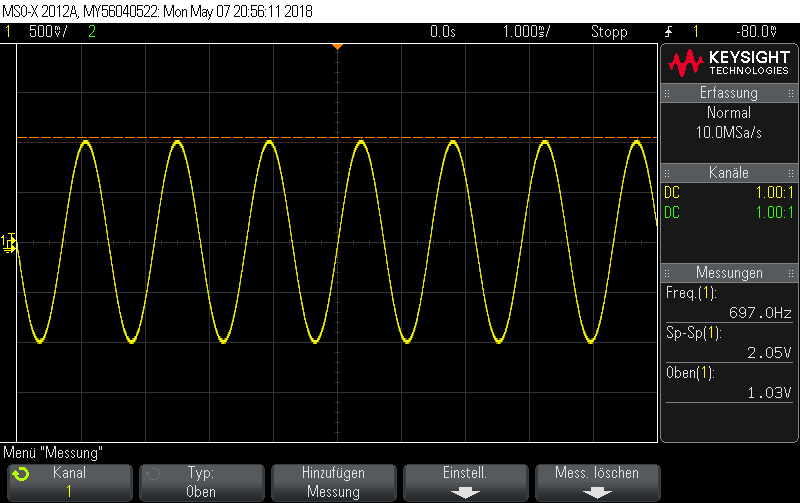
\includegraphics[width=0.8\textwidth]{aufgabe1_meas.png}
    \caption{Bestimmung Frequenz und Amplitude mit der Measure Funktion}
    \label{fig:meas-freq-ampl}
\end{figure}

\begin{figure}[H]
    \centering
    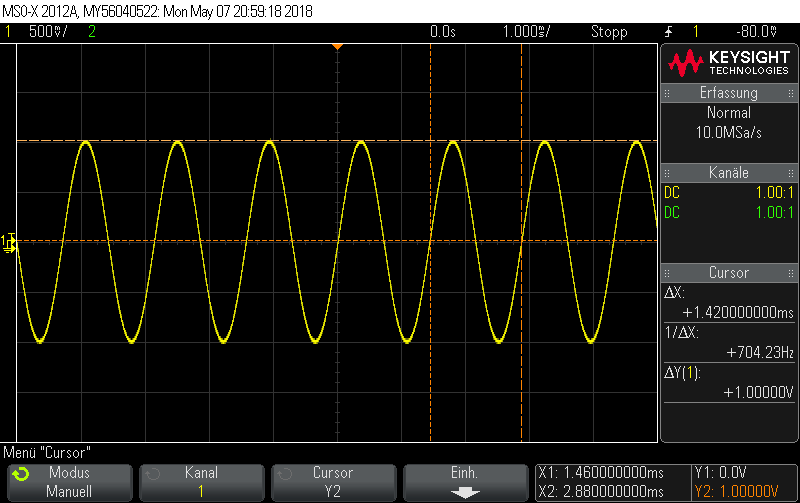
\includegraphics[width=0.8\textwidth]{aufgabe1_cursor.png}
    \caption{Bestimmung Frequenz und Amplitude mit dem Cursor}
    \label{fig:cursor-freq-ampl}
\end{figure}


In Abbildung \ref{fig:cursor-freq-ampl} wird das Signal des Funktionsgenerators dargestellt. Der abgelesene Wert der Amplitude beträgt $\hat{x}=1\si{V}$ und der der Frequenz beträgt $f=697\si{Hz}$. Die Werte stimmen also mit den eingestellten Werten überein.
Der Effektivwert beträgt also $V_\textit{eff}=\frac{\hat{x}}{\sqrt{2}}\approx0,707\si{V}$.

\subsubsection{Fourier-Transformation}
Abbildung \ref{fig:aufgabe1-fft} zeigt die Spektrumsanalyse zu dem Zeitsignal aus dem \hyperref[sec:harmonische-signale]{vorherigen Versuch}.
Der Plot des Spektrums (Abbildung \ref{fig:aufgabe1-fft}) zeigt nur einen Peak bei der  Frequenz $f=697\si{Hz}$. Die Peaks im Plot eigen die Frequenzen, aus denen das analysierte Signal zusammengesetzt ist. Aus dem einzelnen Peak schließen wir, dass das Signal bereits ein harmonisches Sinussignal ist mit der Frequenz $f=697\si{Hz}$.

\begin{figure}[H]
    \centering
    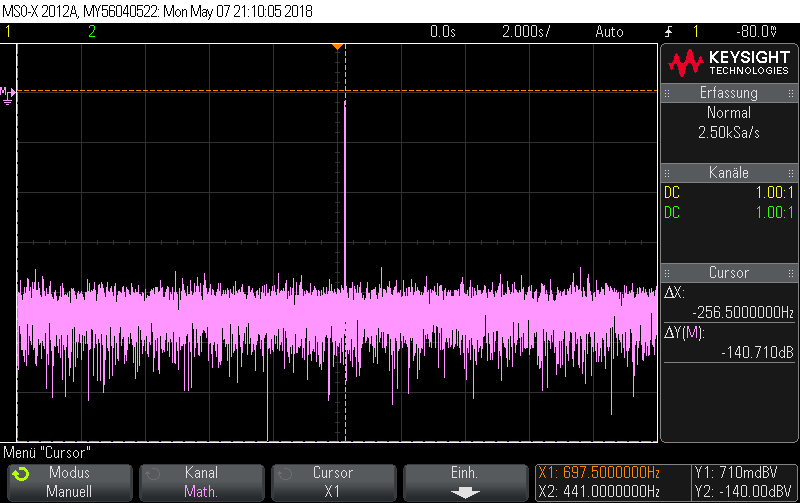
\includegraphics[width=0.8\textwidth]{aufgabe1_fft.png}
    \caption{Fourier Transformation auf Signal angewendet}
    \label{fig:aufgabe1-fft}
\end{figure}

Der ausgegebene Ton klingt unangenehm hoch.

\subsubsection{FFT vs. Gehör}
Für diesen Versuch wurde mit dem internen Frequenzgenerator des Oszilloskops ein Sinussignal der Frequenz $f=1477\si{Hz}$ und einer Amplitude $\hat{x}=1\si{V}$ mit einem Offset $V_{\textit{off}}=100\si{mV}$ erzeugt.

Aus dem Plot der Funktion im Zeitbereich (Abbildung \ref{fig:aufgabe2-time}) kann man eine Amplitude $\hat{x}=1\si{V}$ und ein Offset $V_{\textit{off}}=100\si{mV}$ ablesen. Der Plot der Funktion im Frequenzbereich (Abbildung \ref{fig:aufgabe3-fft}) zeigt nur einen Peak der eingestellten Frequenz $f=1477\si{Hz}$.
Das Offset ist im Frequenzbereich ein Signal der Frequenz null und der Amplitude $V_{\textit{off}}$. Dadurch \glqq verschwindet\grqq\ der Peak des Offsets in der $y$-Achse.

\begin{figure}[H]
    \centering
    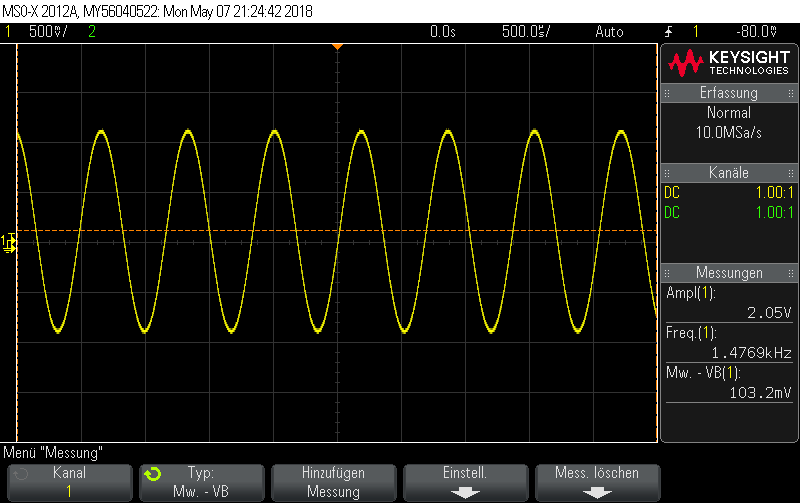
\includegraphics[width=0.8\textwidth]{aufgabe2_time.png}
    \caption{Zeitsignal und Messungen des Signals}
    \label{fig:aufgabe2-time}
\end{figure}

\begin{figure}[H]
    \centering
    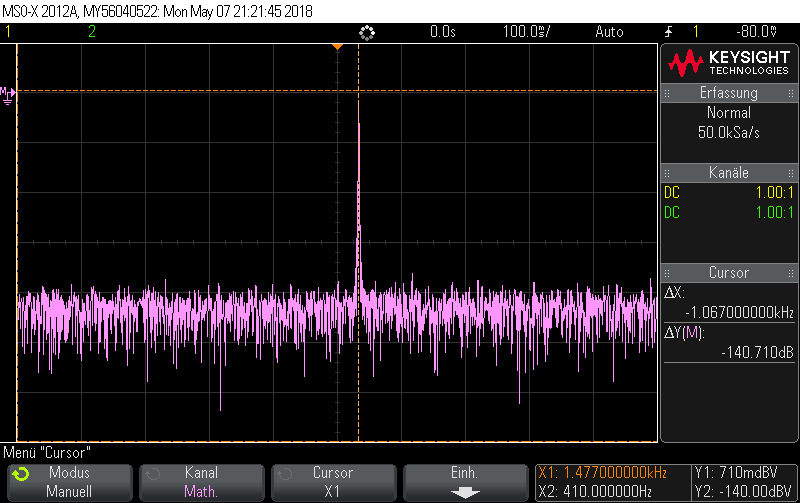
\includegraphics[width=0.8\textwidth]{aufgabe2_fft.png}
    \caption{Fourier Transformation auf Signal angewendet}
    \label{fig:aufgabe2-fft}
\end{figure}

Das Audiosignal klingt wieder unangenehm, allerdings diesmal wesentlich höher.
Als nächtes wurde ein Sinussignal der Frequenz $f=1480\si{Hz}$ und einer Amplitude $\hat{x}=1\si{V}$ erzeugt.
Dieses Signal lässt sich akkustisch nicht von dem vorherigen Signal unterscheiden, da die Differenz der beiden Frequenzen sehr gering ist.

Die Frequenzauflösung $f_{\textit{res}}$ berechnet sich durch:
\begin{equation*}
   f_{\textit{res}}=\frac{1}{t_{\textit{mess}}}\\
\Leftrightarrow t_{\textit{mess}}=\frac{1}{f_{\textit{res}}} 
\end{equation*}
Die Differenz zwischen den beiden Frequenzen beträgt $f_\delta=3\si{Hz}=f_{\textit{res}}$
\begin{equation*}
    t_{\textit{mess}}=\frac{1}{3\si{Hz}}=\frac{1}{3}\si{s}
\end{equation*}
Das Messintervall darf also minimal $t_{\textit{mess}}=\frac{1}{3}\si{s}$ betragen.
Das entspricht bei einer Frequenz $f=1480\si{Hz}$ $N=\frac{t}{T}=t\cdot f \approx 493$ Perioden.


\subsection{Messung periodischer Signale}
Im folgenden wurde der Trigger des Oszilloskops mit einem externen Frequenzgenerator gekoppelt.
Über Kanal $1$ wurde ein gemischtes Signal aus dem externen und dem internen Funktionsgenerators gemessen.

Der externe Funktionsgenerator erzeugt ein Sinussignal der Frequenz $f_\textit{ext}=697\si{Hz}$ bei einer Amplitude $\Hat{x}=1V$ bzw. $V_\textit{SS}=2V$. Die Einstellungen wurden mit dem Oszilloskop überprüft.

Der interne Funktionsgenerator erzeugt ein Sinussignal der Frequenz $f_\textit{int}=1336\si{Hz}$ bei einer Amplitude $\Hat{x}=1V$ und einem Offset $V_\textit{off}=0V$.

Das Signal am Kanal$1$ ist eine Überlagerung beider Funktionen mit unterschiedlichen Frequenzen $f_\textit{ext}$ und $f_\textit{int}$. Dieses überlagerte Signal erzeugt zufällige Punkte an denen der Trigger vermeintlich wiederkehrende Frequenzen erkennt und danach den Trigger einstellt. Diese Triggerpunkte sind nicht konstant, wodurch keine stehende Welle entsteht.

\begin{figure}[H]
    \centering
    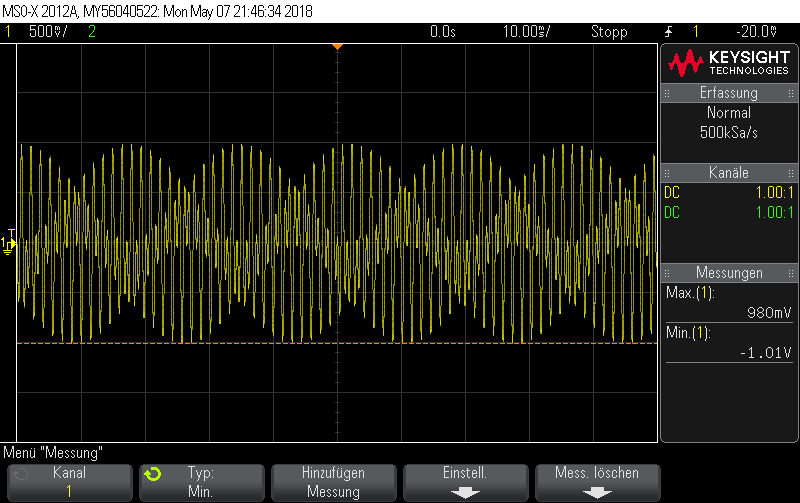
\includegraphics[width=0.8\textwidth]{aufgabe3_time.png}
    \caption{Zeitsignal und Messungen des Signals}
    \label{fig:aufgabe3-meas}
\end{figure}


Der Minimalwert beträgt $V_\textit{min}=-1,01\si{V}$ und der Maximalwert $V_\textit{max}=980\si{mV}$, wie in Abbildung \ref{fig:aufgabe3-meas} zu erkennen.

Es ist ein normaler Ton zu hören, der allerdings aus der Überlagerung zweier Töne besteht.

Im Frequenzdiagramm (Abbildung \ref{fig:aufgabe3-fft}) sind zwei Frequenzen $f_1=697\si{Hz}$ und $f_2=1336\si{Hz}$ in Form zweier Peaks erkennbar. Das Signal am Eingang ist also aus zwei Frequenzen zusammengesetzt

\begin{figure}[H]
    \centering
    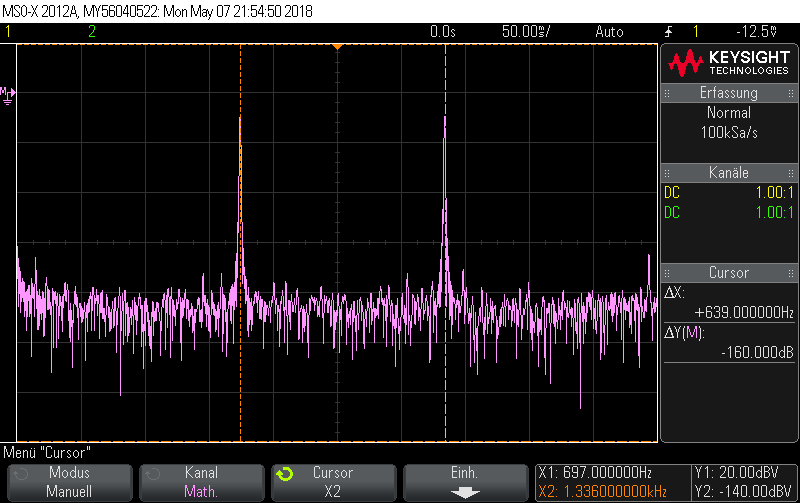
\includegraphics[width=0.8\textwidth]{aufgabe3_fft_band.png}
    \caption{Signal im Frequenzbereich}
    \label{fig:aufgabe3-fft}
\end{figure}

Die obere Grenzfrequenz $f_\textit{grenz,oben}=1336\si{Hz}$ und untere Grenzfrequenz $f_\textit{grenz,unten}=697\si{Hz}$ bilden eine Bandbreite von $f_\textit{band}=639\si{Hz}$.

\subsection{Mehrfrequenzwahlverfahren}
\subsubsection{DTMF-App}

Wenn Tasten in der gleichen Spalte gedrückt werden, bleibt der rechte Peak konstant, der andere wird verschoben, in der gleichen Zeile bleibt der linke Peak gleich, wie in den folgenden Abbildungen \ref{fig:aufgabe4-2} - \ref{fig:aufgabe4-0} ersichtlich.

\begin{figure}[H]
    \centering
    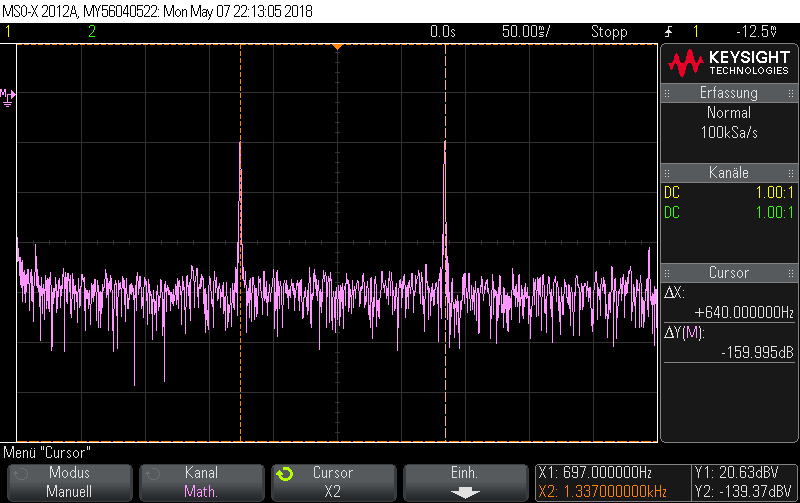
\includegraphics[width=0.8\textwidth]{aufgabe4_2.png}
    \caption{Signal beim Drücken von \glqq 2\grqq: $697\si{Hz}, 1337\si{Hz}$}
    \label{fig:aufgabe4-2}
\end{figure}

\begin{figure}[H]
    \centering
    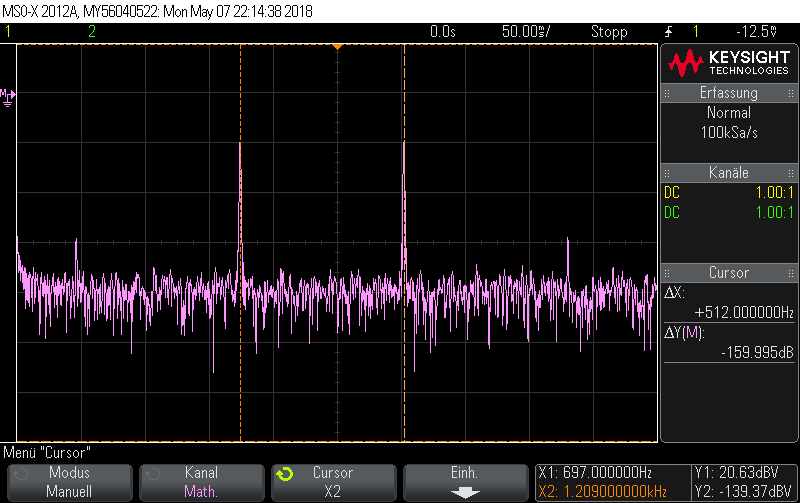
\includegraphics[width=0.8\textwidth]{aufgabe4_1.png}
    \caption{Signal beim Drücken von \glqq 1\grqq: $697\si{Hz}, 1209\si{Hz}$}
    \label{fig:aufgabe4-1}
\end{figure}

\begin{figure}[H]
    \centering
    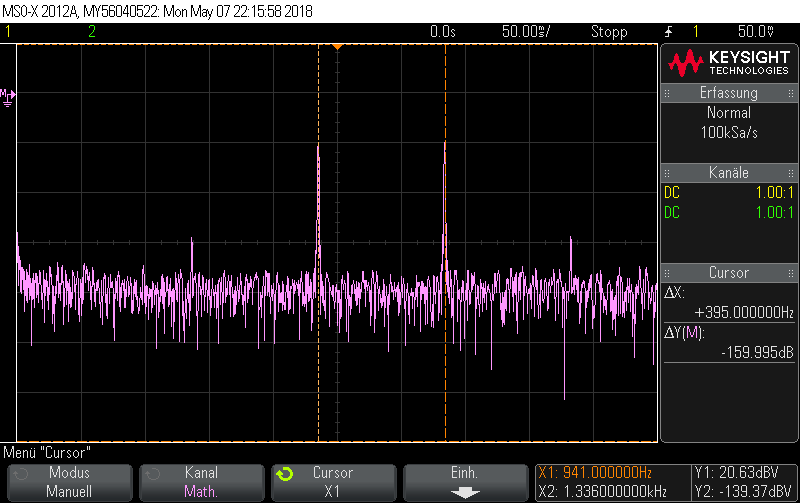
\includegraphics[width=0.8\textwidth]{aufgabe4_0.png}
    \caption{Signal beim Drücken von \glqq 0\grqq: $941\si{Hz}, 1336\si{Hz}$}
    \label{fig:aufgabe4-0}
\end{figure}

\subsubsection{Sourcecode}
Folgende Code-Zeilen wurden verändert, damit \lstinline{generate_tones()} korrekt funktioniert:
\begin{lstlisting}
%Frequenz horizontal (Zeilenvektor)
fhorz = [ 1209, 1336, 1477 ];

%Frequenz vertikal (Zeilenvektor)
fvert = [ 697, 770, 852, 941 ];

(...)

Ton1 = cos(2*pi*f1*t);
Ton2 = cos(2*pi*f2*t);

tone=(Ton1+Ton2)/2;
\end{lstlisting}

\subsubsection{FFT Tastentöne}
Der folgende Versuch ist eine reine Simulation in der Matlab-Umgebung.
Über die Funktion \lstinline{dial_tones()} wurde das Signal für die Taste \glqq$1$\grqq erzeugt.
Die beiden Auftretenden Frequenzen sind $f_1=697\si{Hz}$ und $f_2=1209\si{Hz}$.

\begin{figure}[H]
    \centering
    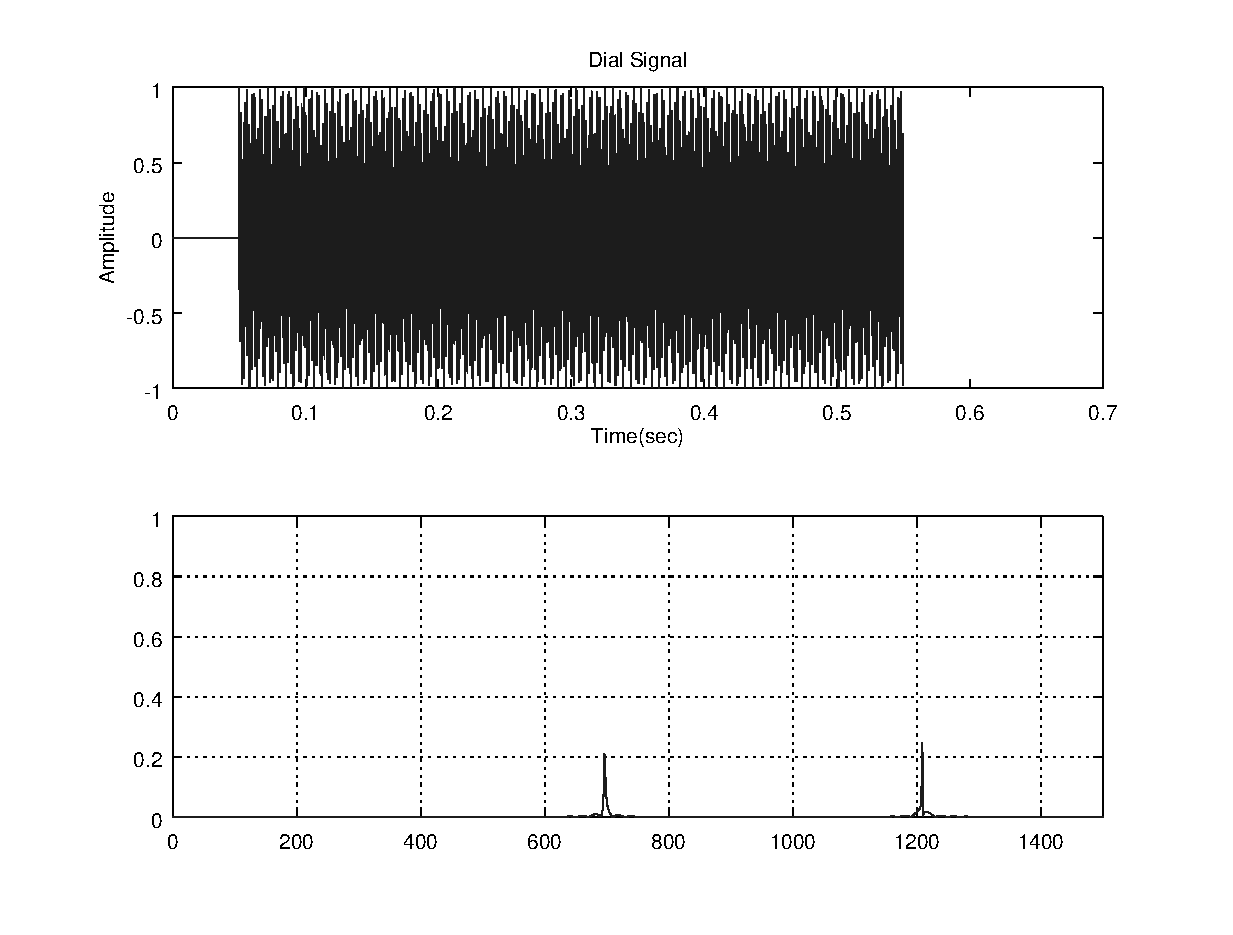
\includegraphics[width=0.8\textwidth, keepaspectratio]{nummer_1_fft.eps}
    \caption{Frequenz- und Zeitbereich: 1}
    \label{fig:nummer-1-fft}
\end{figure}

Im zweiten Versuch wurde das Signal für die Taste \glqq$5$\grqq erzeugt.
Die beiden Auftretenden Frequenzen sind $f_1=770\si{Hz}$ und $f_2=1336\si{Hz}$.

\begin{figure}[H]
    \centering
    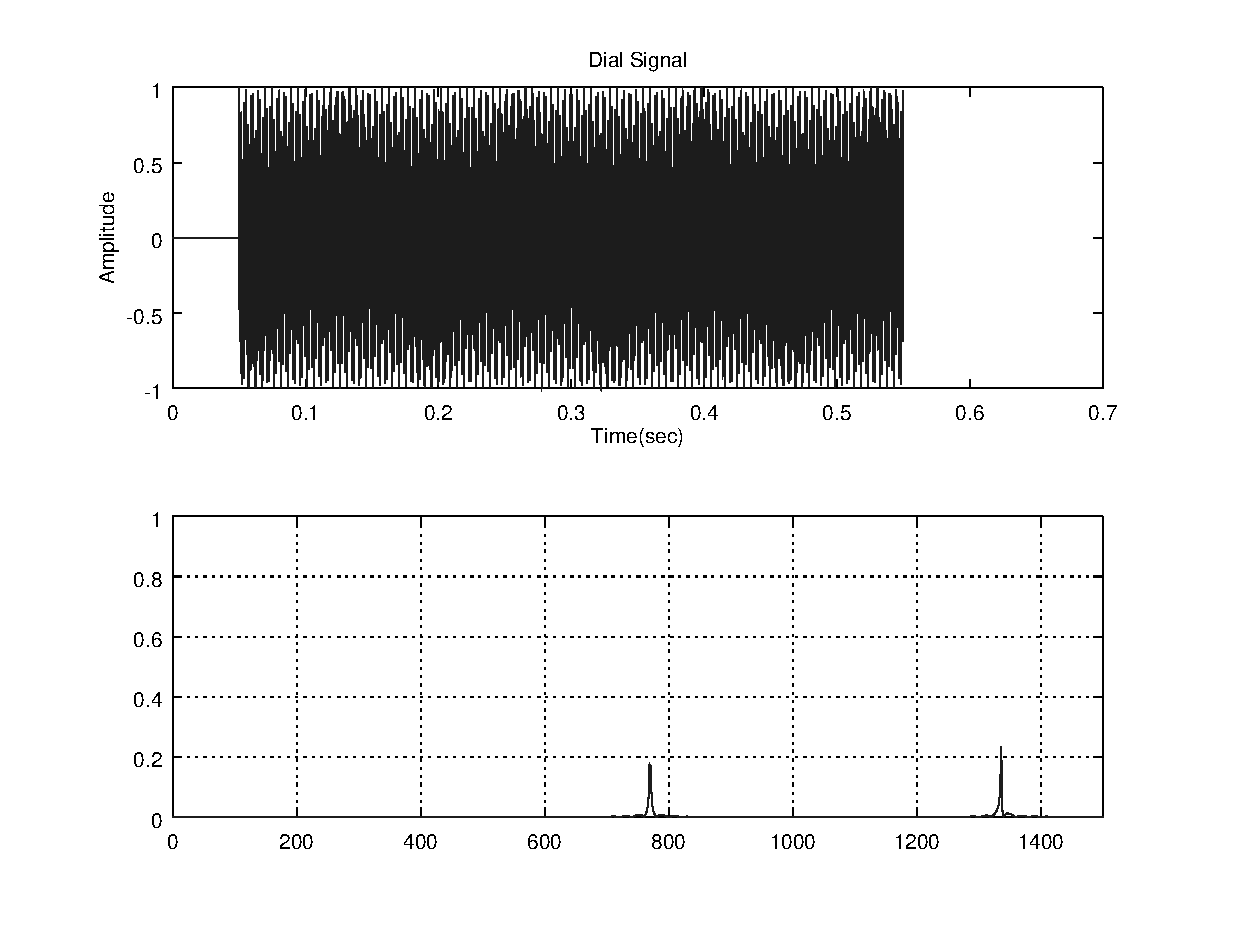
\includegraphics[width=0.8\textwidth, keepaspectratio]{nummer_5_fft_time.eps}
    \caption{Frequenz- und Zeitbereich: 5}
    \label{fig:nummer-5-fft-time}
\end{figure}

Zuletzt wurde das Signal für die Taste \glqq$9$\grqq erzeugt.
Die beiden Auftretenden Frequenzen sind $f_1=941\si{Hz}$ und $f_2=1477\si{Hz}$.

\begin{figure}[H]
    \centering
    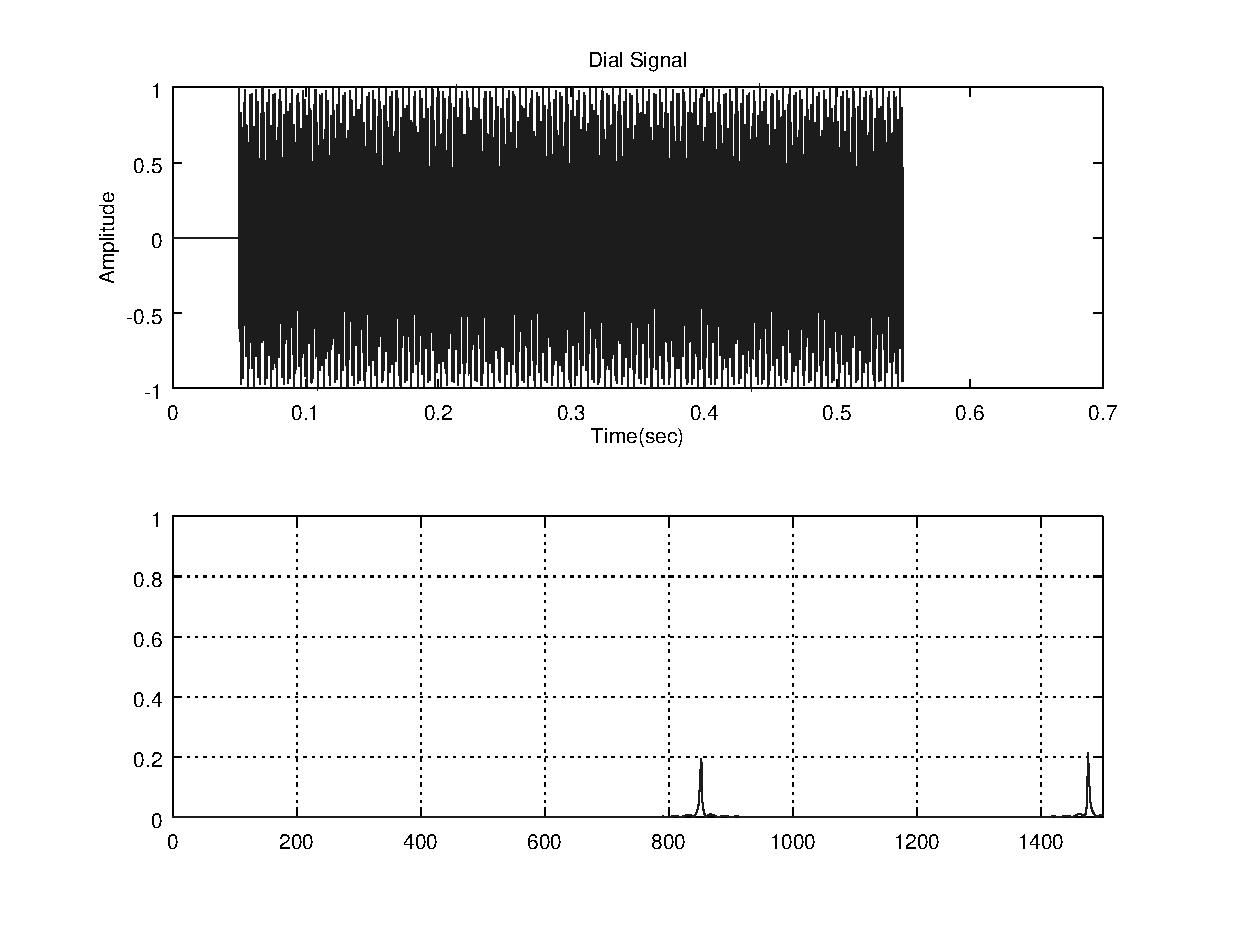
\includegraphics[width=0.8\textwidth, keepaspectratio]{nummer_9_fft_time.eps}
    \caption{Frequenz- und Zeitbereich: 9}
    \label{fig:nummer-9-fft-time}
\end{figure}

\subsubsection{Identifikation einer unbekannten Nummer}
In diesem Versuch wurde eine unbekannte $12$-stellige Telefonnummer aus der Datei \lstinline{dialed_number.mat} ermittelt. 
Zuerst wurde mithilfe der Funktion \lstinline{soundsc(dialed_number.mat,32786)} aus dieser Datei eine Tonwiedergabe generiert. Der zweite Parameter in der Funktion ist dabei die Abtastrate.\\

Um das gesamte Signal darstellen zu können, musste der Code der Funktion \lstinline{fft_dtmf.m} vervollständigt werden.
Der vervollständigte Code der Funktion sieht folgendermaßen aus:

\begin{lstlisting}
%Signal im Zeitbereich
time = [0:length(tones)-1]/Fs;
plot(time,tones);

(...)

%Transformation in den Frequenzbereich
plot(f,abs(fft(tones))/(Fs/2));
\end{lstlisting}

Es ist nicht möglich mittels Fouriertransformation über das gesamte Signal die gewählte Nummer zu ermitteln, da die Nummern mehrfach aus den gleichen Frequenzen in jeweils unterschiedlichen Kombinationen zusammengesetzt werden.
Die ermittelten Frequenzen aus der Fouriertransformation wären dann nicht eindeutig bestimmten Nummern zuzuordnen.
Stattdessen kann man die kurzen Pausen zwischen den Tönen als Intervallgrenzen verwenden und dann für jedes Intervall mithilfe der Fouriertransformation die zusammengesetzten Frequenzen bestimmen.\\

Unter Verwendung der Funktion \lstinline{recieve_dial} wurden nun die Frequenzen und die dazugehörende Nummer bestimmt.
Im folgenden werden drei der vorkommenden Ziffern exemplarisch analysiert.

\begin{figure}[H]
    \centering
    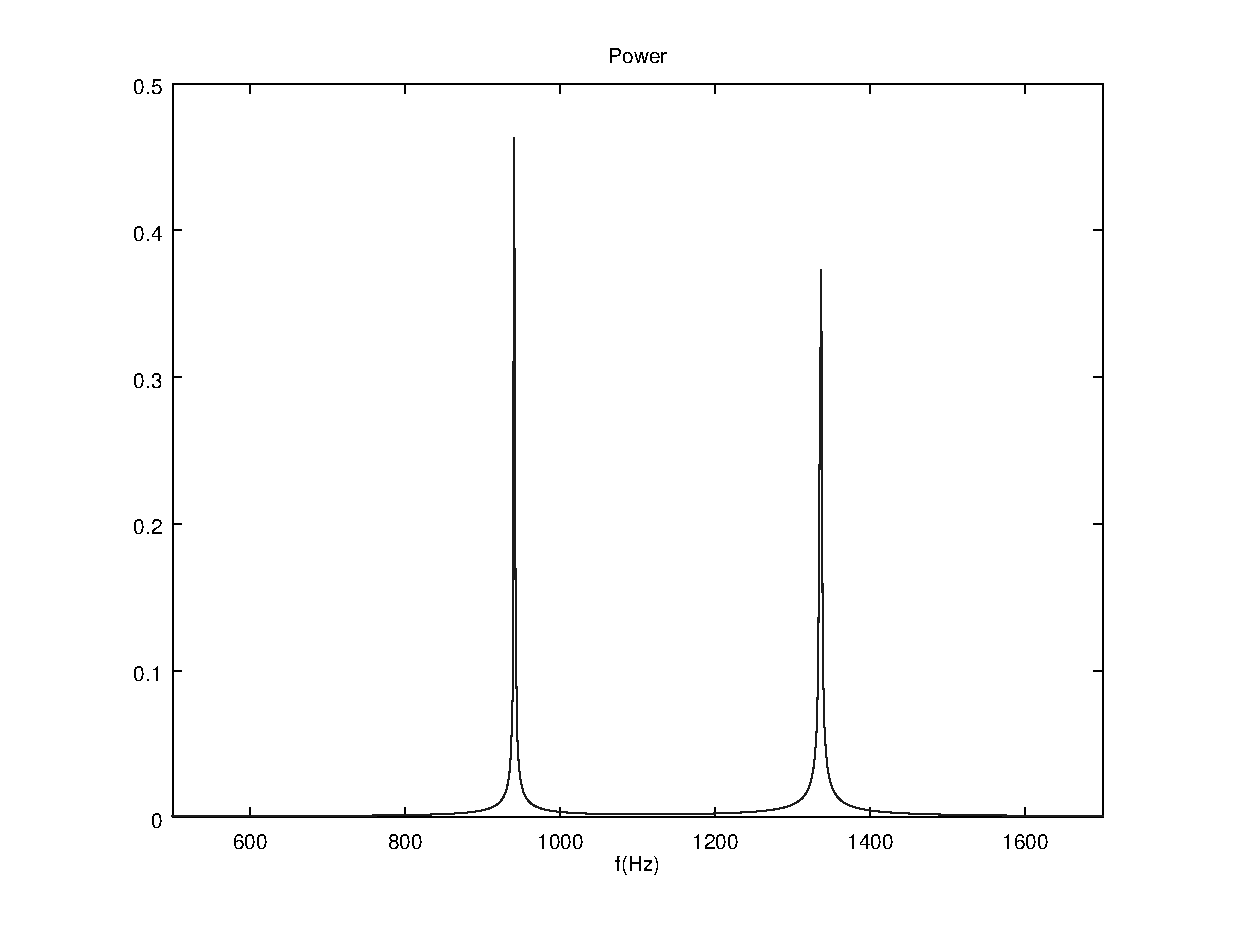
\includegraphics[width=0.8\textwidth, keepaspectratio]{nummer_0_fft.eps}
    \caption{Frequenzbereich: 0}
    \label{fig:nummer-0-fft}
\end{figure}

Abbildung \ref{fig:nummer-0-fft} zeigt die Fouriertransformation an der Stelle. Es treten die Frequenzen $f_1\approx950\si{Hz}$ und $f_2\approx1350\si{Hz}$. Die gewählte Ziffer an dieser Stelle ist also 0.

\begin{figure}[H]
    \centering
    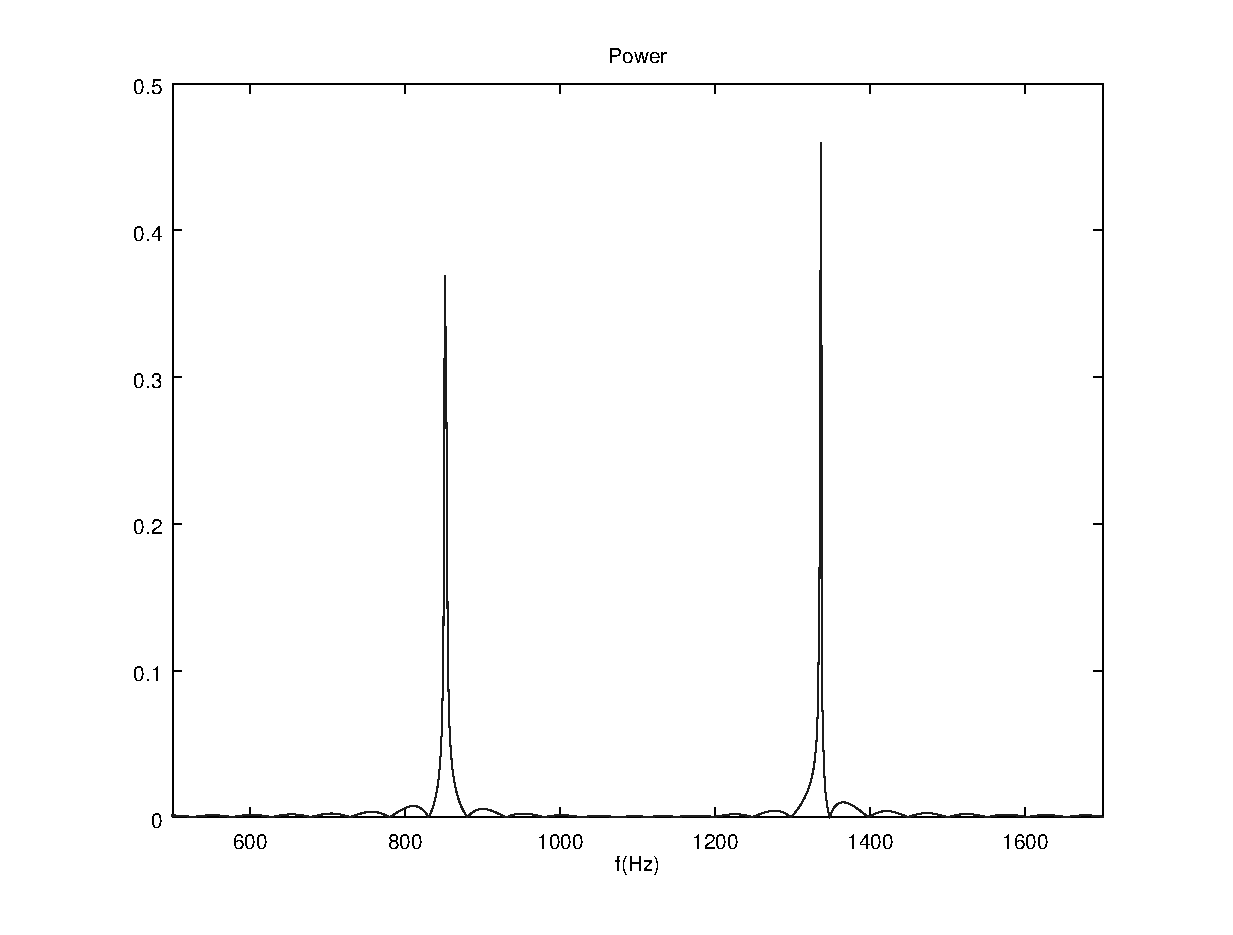
\includegraphics[width=0.8\textwidth, keepaspectratio]{nummer_8_fft.eps}
    \caption{Frequenzbereich: 8}
    \label{fig:nummer-8-fft}
\end{figure}

Abbildung \ref{fig:nummer-8-fft} zeigt die Fouriertransformation an der Stelle. Es treten die Frequenzen $f_1\approx850\si{Hz}$ und $f_2\approx1340\si{Hz}$. Die gewählte Ziffer an dieser Stelle ist also 8.

\begin{figure}[H]
    \centering
    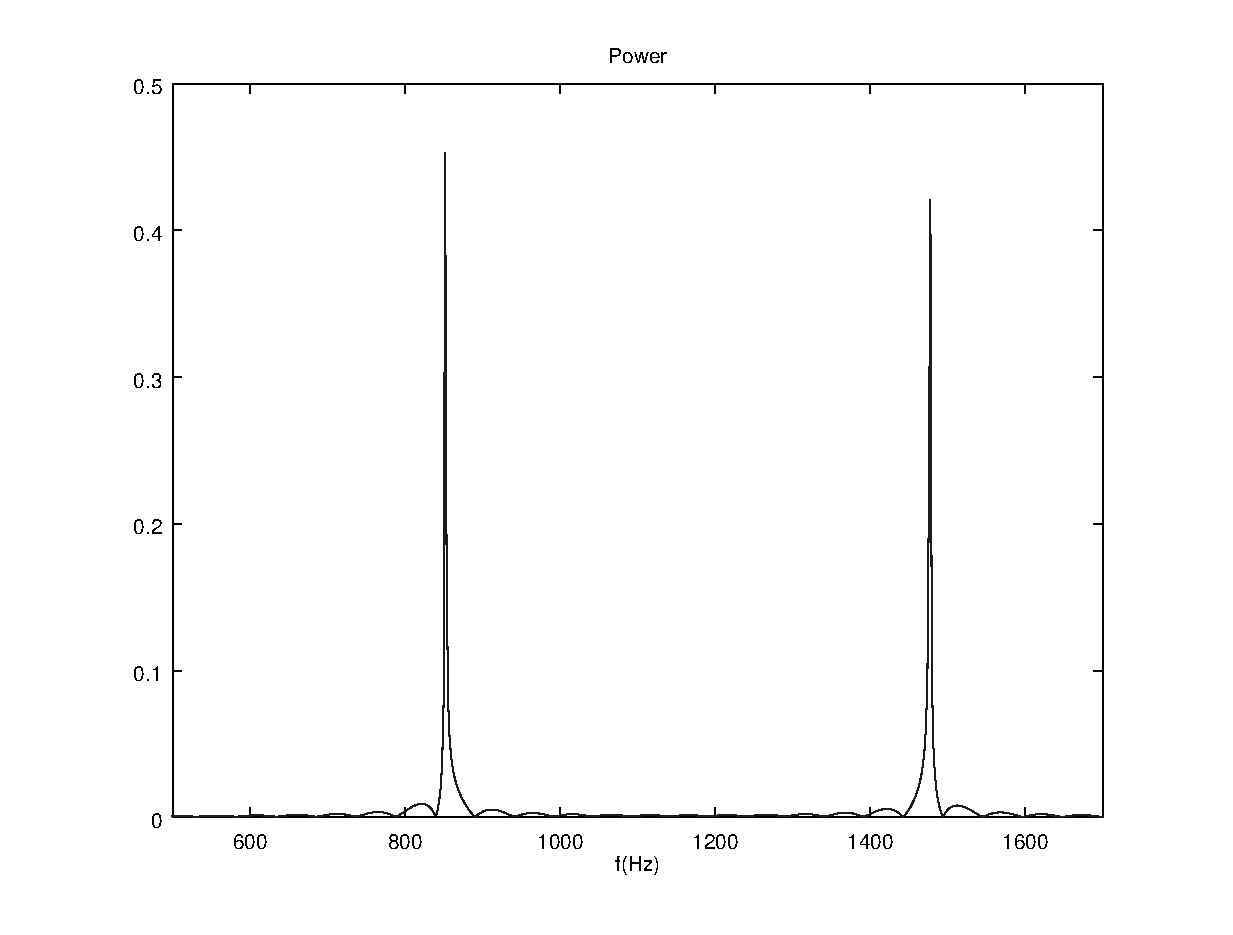
\includegraphics[width=0.8\textwidth, keepaspectratio]{nummer_9_fft.eps}
    \caption{Frequenzbereich: 9}
    \label{fig:nummer-9-fft}
\end{figure}

Abbildung \ref{fig:nummer-9-fft} zeigt die Fouriertransformation an der Stelle. Es treten die Frequenzen $f_1\approx850\si{Hz}$ und $f_2\approx1480\si{Hz}$. Die gewählte Ziffer an dieser Stelle ist also 9.

Diese Verfahren wurde auf jedes Intervall angewendet. Dadurch ergibt sich folgende zwölfstellige Telefonnummer: 089452356700

Die Funktion \lstinline{receive_dial} berechnet in Zeile $16$ die Fouriertransformation der einzelnen Zeitabschnitte. Ab Zeile $26$ wird das Ergebnis der jeweiligen Zeile und Spalte auf dem Numpad zugeordnet.
\end{document}
